% \documentclass[14pt,a4paper]{report}
\documentclass[14pt,a4paper]{article}
\usepackage[utf8]{inputenc}
\usepackage[english,vietnamese]{babel}
\usepackage[left=3.50cm, right=2.00cm, top=2.00cm, bottom=2.00cm]{geometry}
\usepackage{multirow}
\usepackage{listings}
\lstset{basicstyle=\ttfamily,escapechar=\@}
\usepackage{paralist}
\usepackage{graphicx}
\usepackage{wrapfig}
\usepackage{setspace}
\usepackage{amsthm}
\usepackage{array}
\usepackage{hyperref}
\hypersetup{colorlinks=true,pdfencoding=auto}
\usepackage{hypcap}
\usepackage{longtable}
\usepackage{rotating}
\usepackage{subfig}
\usepackage{float}
\renewcommand{\baselinestretch}{1.3}
\usepackage{indentfirst}
\usepackage{pgfgantt}
\usepackage{amsmath}
\selectlanguage{vietnamese}

\begin{document}

\begin{titlepage}
\begin{center}

\vspace*{3\bigskipamount}

\begin{otherlanguage*}{vietnamese}
\makeatletter
\fontsize{12}{12}\textbf{ĐẠI HỌC QUỐC GIA TP HỒ CHÍ MINH}\\
\fontsize{14}{14}\textbf{TRƯỜNG ĐẠI HỌC BÁCH KHOA}\\
\fontsize{14}{14} -----------------------------------
\makeatother

\begin{figure}[h]
	\centering
		
\includegraphics[width=0.4\columnwidth]{./title/bach_khoa.jpeg}
		\centering
	\label{fig:logo}
\end{figure}

{\makeatletter
\fontsize{16}{16}\textbf{Trần Hoàng Tuấn}\\
\makeatother}

\vspace{1.2cm}

{\makeatletter
\fontsize{18}{18}\textbf{SINH BIỂU CẢM KHUÔN MẶT DỰA TRÊN PHÙ HỢP GIỌNG NÓI}\\
\makeatother}

\vspace{1.2cm}
{\makeatletter
\fontsize{18}{18}\textbf{ĐỀ CƯƠNG LUẬN VĂN THẠC SĨ}\\
\makeatother}


\vspace{8cm}
{\makeatletter
\fontsize{12}{12} HỒ CHÍ MINH - 2020\\
\makeatother}

\end{otherlanguage*}

\end{center}
\end{titlepage}


\begin{titlepage}

\begin{center}

\vspace*{3\bigskipamount}

\begin{otherlanguage*}{vietnamese}

\makeatletter
\fontsize{12}{12}\textbf{ĐẠI HỌC QUỐC GIA TP HỒ CHÍ MINH}
\makeatother

\makeatletter
\fontsize{14}{14}\textbf{TRƯỜNG ĐẠI HỌC BÁCH KHOA}\\
\fontsize{14}{14} -----------------------------------
\makeatother

\begin{figure}[h]
	\centering
		
\includegraphics[width=0.4\columnwidth]{./title/bach_khoa.jpeg}
		\centering
	\label{fig:logo}
\end{figure}

{\makeatletter
\fontsize{16}{16}\textbf{TRẦN HOÀNG TUẤN}
\makeatother}

\vspace{1cm}

{\makeatletter
\fontsize{16}{16}\textbf{SINH BIỂU CẢM KHUÔN MẶT DỰA TRÊN PHÙ HỢP GIỌNG NÓI}\\
\vspace{1cm}
\fontsize{12}{12} NGÀNH: KHOA HỌC MÁY TÍNH\\
\fontsize{12}{12} MÃ NGÀNH: 60.48.01.01\\
\makeatother}

\vspace{1cm}
{\makeatletter
\fontsize{12}{12}\textbf{ĐỀ CƯƠNG LUẬN VĂN THẠC SĨ}\\
\makeatother}

\vspace{1cm}
{\makeatletter
\fontsize{12}{12}\textbf{NGƯỜI HƯỚNG DẪN KHOA HỌC}\\
\fontsize{12}{12}\textbf{TIẾN SĨ: LÊ THÀNH SÁCH}\\
\makeatother}

\vspace{4cm}
{\makeatletter
\fontsize{12}{12} HỒ CHÍ MINH - 2020\\
\makeatother}

\end{otherlanguage*}

\vfill
\end{center}
\end{titlepage}



\pagenumbering{gobble}
\tableofcontents
\listoffigures

\pagenumbering{arabic}
\section{\texorpdfstring{Giới thiệu đề tài}{Introduce}}
Bài toán tạo sinh dữ liệu dựa trên những nguồn dữ liệu có tính chất khác nhau đã và đang trở thành xu thế trong những năm trở lại đây. Đây là bài toán có tính cấp bách, mang lại giá trị cao về mặt kiến thức cho ngành trí tuệ nhân tạo nói riêng và giá trị về mặt kinh tế, công nghệ chung cho toàn xã hội xã hội. Bên cạnh đó, việc tạo sinh dữ liệu về con người đã đạt được những tiến bộ vượt bậc, đặc biệt là tạo sinh dữ liệu hình ảnh khuôn mặt người. Trong để tài này, mục đích nghiên cứu là: cho biết một vài dữ liệu về gương mặt của một người bất kỳ (hình ảnh, video ngắn) và một đoạn tiếng nói bất kỳ, tạo sinh hình ảnh khuôn mặt người đó đang nói đoạn tiếng nói đã cho một cách chân thực.

Ý nghĩa khoa học: Đóng góp cho sự phát triển chung của xu hướng tạo sinh dữ liệu mới dựa trên các tính chất của dữ liệu ban đầu. Việc tìm ra phương pháp giải quyết tốt bài toán sẽ tạo nên tảng để giải quyết những bài toán xa hơn, phức tạp hơn như: tạo sinh nửa người trên, tạo sinh toàn bộ cơ thể người, hay tạo sinh cả một bối cảnh trong phim. Đề tài giúp hiện thực, cải tiến các phương pháp hiện có trong các bài nghiên cứu gần đây, so sánh và cải tiến để cho ra kết quả tạo sinh tốt hơn, đóng góp thêm phương pháp mới cho việc tạo sinh ảnh. Đồng thời, các phương pháp tạo sinh dữ liệu cũng giúp làm giàu dữ liệu để huấn luyện, kiểm thử cho các mô hình học máy, học sâu khác.

Ý nghĩa thực tiễn: Giải quyết thành công vấn đề này đem lại giá trị to lớn về mặt công nghệ, kinh tế và xã hội. Chúng ta có thể tái hiện lại gương mặt người đang nói ở nhiều thứ tiếng khác nhau, tạo sinh khuôn mặt người đại diện trong các hội nghị trực tuyến, tích hợp vào các trò chơi điện tử để làm chúng trở nên chân thực hơn, truyền video trong điều kiện băng thông giới hạn, giả lập trợ lý ảo có hình dáng con người,... Đối với ngành truyền thông, nó có thể tạo ra biên tập viên ảo. Đối với ngành điện ảnh, giải trí, sáng tạo nội dung nó cũng có giá trị ứng dụng khi giúp giảm bớt áp lực lên khâu hóa trang, kỹ xảo.

Kiến trúc mạng Generative Adversarial Network \cite{gans_base} ra đời vào năm 2014 đã đánh dấu một bước chuyển mình mới cho ngành trí tuệ nhân tạo. Kiến trúc này giúp cho việc tạo sinh dữ liệu được thực hiện một cách hiệu quả và chính xác hơn. Dựa trên nền tảng đó, các nghiên cứu về việc tạo sinh ảnh gương mặt người cũng được tiến hành và ngày càng có những bước tiến mới. 

Để tạo sinh mặt người đang nói, các công trình nghiên cứu tập trung chủ yếu vào vùng miệng. Bài nghiên cứu vào năm 2018 của Lele Chen \cite{chen2018} đưa ra phương pháp tạo sinh video vùng miệng của người đang nói với đầu vào là ảnh tĩnh của khuôn miệng và một đoạn âm thanh có chứa tiếng nói. Vào năm 2019, Lele Chen \cite{chen2019} và Vougioukas \cite{vougioukas2019} tiếp tục đưa ra phương pháp tạo sinh cả khuôn mặt người dựa vào ảnh tĩnh của khuôn mặt và đoạn âm thanh chứa tiếng nói. Năm 2020, Vougioukas \cite{vougioukas2020} đã cải tiến phương pháp tạo sinh mặt và cập nhật thêm hành động chớp mắt, Lele Chen \cite{chen2020} cũng đưa ra phương pháp mới để tạo sinh mặt hiệu quả hơn, tự nhiên hơn với việc di chuyển của vùng đầu trên khung hình.
 
Nhìn chung, các nghiên cứu này đã đưa ra các kiến trúc mạng hiệu quả để tạo sinh khuôn mặt cũng như các phương pháp, lập luận và chứng minh tính hiệu quả của các kiến trúc mạng được đề xuất. Mặc dù các thông số của thử nghiệm đưa ra là khá tốt, các nghiên cứu của Vougioukas vẫn chưa thể tạo ra chuyển động của đầu, kết quả tạo sinh của Vougioukas đôi khi không giữ được đặc trưng của ảnh. Nghiên cứu của Lele Chen năm 2020 \cite{chen2020} đã tạo ra chuyển động cho phần đầu dựa trên tiếng nói, nhưng khuôn mặt được tạo sinh vẫn còn có thể bị nhận ra qua các phép thử Turing, và chuyển động của đầu đôi khi vẫn chưa được tự nhiên, mạng cũng có cấu trúc rất phức tạp và đòi hỏi nhiều tài nguyên tính toán để có thể huấn luyện.

\section{\texorpdfstring{Mục tiêu, giới hạn và đối tượng nghiên cứu}{Target, limitation}}
\subsection{\texorpdfstring{Mục tiêu}{Target}}
Mục tiêu của Luận văn Tốt nghiệp là nghiên cứu các đề tài có liên quan bằng cách khảo sát, kiểm định và thử nghiệm các nghiên cứu mới nhất hiện có, qua đó tiến hành các cải tiến, thay đổi và thử nghiệm để đưa ra các kết quả tạo sinh khuôn mặt tốt hơn, tự nhiên hơn, chính xác hơn. Hình ảnh được tạo ra phải sắc nét, ít nhiễu, chân thực và tương đồng về mặt nhận dạng, cấu trúc với hình ảnh người mẫu. Đồng thời, khẩu hình miệng của hình ảnh được tạo ra phải khớp với tiếng nói. Bên cạnh đó, video được tạo ra phải có tính liền lạc, ổn định, không bị hiện tượng nhảy hình. Mục tiêu được đặt ra nhằm cải thiện các mô hình hiện có, tăng tính ứng dụng của việc tạo sinh mặt người vào thực tiễn cuộc sống.

\subsection{\texorpdfstring{Giới hạn}{Limitation}}
Phạm vi nghiên cứu của Luận văn là tạo sinh ảnh giới hạn trong vùng mặt của người, dữ liệu mẫu được cung cấp ban đầu phải là ảnh rõ ràng của khuôn mặt người, đoạn âm thanh được cung cấp cũng phải là âm thanh rõ ràng của tiếng nói cùng loại với ngôn ngữ được dùng để huấn luyện mạng.

\subsection{\texorpdfstring{Đối tượng nghiên cứu}{Research}}
Đối tượng nghiên cứu của Luận văn là các cách tiếp cận, các phương pháp mô hình hóa bài toán, các mạng học máy, học sâu, mạng GANs và các phương pháp tạo sinh dữ liệu từ mạng GANs, các cấu trúc Residual Encoder-Decoder, bên cạnh đó là các phương pháp kết hợp đặc trưng hình ảnh, âm thanh có xem xét đến thứ tự thời gian để tạo sinh hình ảnh mới.

\subsection{\texorpdfstring{Kết quả dự kiến}{Result}}
Luận văn sẽ xây dựng được mô hình tính toán mới để có thể tạo sinh hình ảnh mặt người hiệu quả, thỏa mãn được các tiêu chí đã nêu trong phần đầu. Đồng thời, luận văn cũng sẽ cung cấp được các đánh giá và so sánh khách quan bằng số liệu thực tế.

\section{\texorpdfstring{Phương pháp nghiên cứu}{Method}}
\subsection{\texorpdfstring{Phương pháp đánh giá kết quả nghiên cứu}{Empty}}
Do đặc thù của bài toán là tạo sinh ảnh mặt người, việc lựa chọn phương pháp để đánh giá chất lượng và độ chân thật của hình ảnh được tạo ra là một thách thức lớn. Dựa trên các tiêu chí về mặt hình ảnh được đưa ra ở phần \ref{target_label}, đoạn còn lại của phần này sẽ đưa ra các độ đo để đo lường chất lượng hình ảnh của mô hình.

Về chất lượng hình ảnh, hầu hết các nghiên cứu trước đây \cite{chen2018}\cite{chen2019}\cite{vougioukas2019}\cite{vougioukas2020} đều sử dụng \textit{Peak Signal-to-Noise Ratio (PSNR)} và \textit{Structural Similarity Index (SSIM)} như các độ đo để đo lường chất lượng hình ảnh được tạo sinh. Tuy nhiên, PSRN lại không phải là một thông số lý tưởng để đo lường khi nó không quan tâm đến các đặc trưng mặt người trong ảnh. Trong khi đó, SSIM lại là một độ đo tốt hơn khi nó có khả năng đo sự tương đồng về mặt nội dung trong ảnh. SSIM có khả năng so sánh các điểm ảnh và các điểm lân cận của chúng trên ảnh được tạo sinh tương ứng với các điểm trên ảnh thật dựa trên ba tính chất - độ tương phản, độ sáng và cấu trúc. Độ nét cũng là một yếu tố quan trọng nói lên chất lượng ảnh. Độ đo Cummulative Probability Blur Detection được sử dụng trong các nghiên cứu \cite{chen2018}\cite{vougioukas2019}\cite{vougioukas2020}
cũng là một độ đo tốt để đánh giá độ nét của ảnh được tạo sinh.

Để đánh giá việc duy trì nhận dạng người trong các hình ảnh được tạo sinh, \textit{Cosin Similarity (CSIM)} là độ đo được sử dụng để đo lường sự sai lệch về nhận dạng trong ảnh được tạo sinh và ảnh thật. Độ đo này đo lường khoảng cách giữa hai vector đặc trưng của hai ảnh thật và tạo sinh, từ đó cho ra một con số cụ thể về sự sai khác giữa hai ảnh.

Sự phù hợp của khẩu hình miệng với từ ngữ được nói ra cũng là một yếu tố quyết định đối với chất lượng ảnh được tạo sinh. Hiện tại, các nghiên cứu đã đưa ra các độ đo khác nhau để đánh giá sự phù hợp này. Trong \cite{vougioukas2019}\cite{vougioukas2020}, tác giả sử dụng độ đo \textit{Word Error Rate (WER)}, trong nghiên cứu này, video mặt người sinh ra được đưa vào LipNet - một mô hình mạng học sâu để đọc từ từ khẩu hình miệng, các từ được đọc ra được so sánh với từ gốc và tính ra tỉ lệ sai. Lele Chen \cite{chen2018} đã đưa ra một độ đo khác để đo lường sự phù hợp khẩu hình miệng là \textit{Landmark Distance (LMD)} nhằm đo lường khoảng cách Euclide giữa các điểm cấu thành khẩu hình miệng trong ảnh thật và ảnh được tạo sinh.

Các độ đo nêu trên là các độ đo đã được kiểm nghiệm tính hiệu quả trong các nghiên cứu gần đây về tạo sinh mặt người dựa vào tiếng nói. Luận văn có thể kế thừa các độ đo này để đánh giá kết quả nghiên cứu, đồng thời có thể dễ dàng so sánh kết quả nghiên cứu của Luận văn với các kết quả nghiên cứu trước đây.

\subsection{\texorpdfstring{Phương pháp thu thập và phân tích số liệu}{Empty}}
Nhằm mục đích dễ dàng cho việc nghiên cứu, đánh giá và so sánh kết quả với các nghiên cứu trước đây, Luận văn sẽ sử dụng các bộ dữ liệu có sẵn, đã được sử dụng trong các nghiên cứu gần đây có cùng chủ đề. Một số tập dữ liệu sau sẽ được sử dụng trong Luận văn:

\textit{GRID}\cite{grid}: Được công bố vào năm 2006, GRID là một tập dữ liệu miễn phí nhằm phục vụ mục đích nghiên cứu. Tập dữ liệu chứa video của 34 người (18 nam, 16 nữ), 1000 video mỗi người, mỗi video có độ dài 3 giây và trong video này, người nói chỉ nói một câu duy nhất.

\textit{CREMA-D}\cite{crema-d}: Được công bố vào năm 2014, CREMA-D là một tập dữ liệu được cung cấp miễn phí cho mục đích nghiên cứu. CREMA-D chứa 7,442 video từ 91 diễn viên, gồm 48 nam và 43 nữ, độ tuổi từ 20 đến 74 từ các chủng tộc người khác nhau. Mỗi diễn viên sẽ nói 12 câu khác nhau, với mỗi câu, họ sẽ thể hiện 6 loại cảm xúc khác nhau khi nói (giận dữ, chán ghét, sợ hãi, vui vẻ, bình thường, và buồn) và 4 cấp độ cảm xúc (thấp, trung bình, cao, và không xác định).

\textit{LRW}\cite{lrw}: Là một bộ dữ liệu lớn được thu thập từ kênh truyền hình BBC, LRW chứa đến hơn 1000 giờ video người đang nói, với bộ từ điển hơn 1000 từ vựng, hơn 1 triệu từ đã được nói bởi hơn 1000 người khác nhau.

\textit{VoxCeleb}\cite{vox}: Tập dữ liệu chứa hơn 100000 từ được nói bởi 1251 người nổi tiếng, những video này được cắt ra từ các video được tải lên YouTube. Tập dữ liệu cũng cân bằng về mặt giới tính với 55\% video là nam. Nhân vật trong video đến từ nhiều chủng tộc khác nhau, ngữ điệu khác nhau, ngành nghề và lứa tuổi cũng khác nhau. Video trong tập dữ liệu cũng được thu thập trong nhiều hoàn cảnh khác nhau (trên thảm đỏ, sân vận động, trong phòng thu,...) và tất cả các video đều được ghi bằng các thiết bị cầm tay.

\begin{figure}[H]
    \centering
    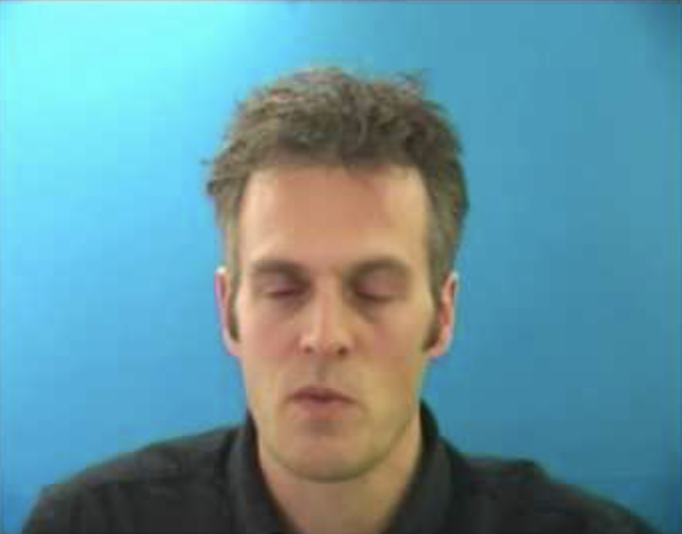
\includegraphics[width=7cm]{./content/images/grid_img.png}
    \caption{Ảnh được cắt từ một video trong tập dữ liệu \textit{GRID}}
    \label{fig:sample-rapv1}
\end{figure}

\begin{figure}[H]
    \centering
    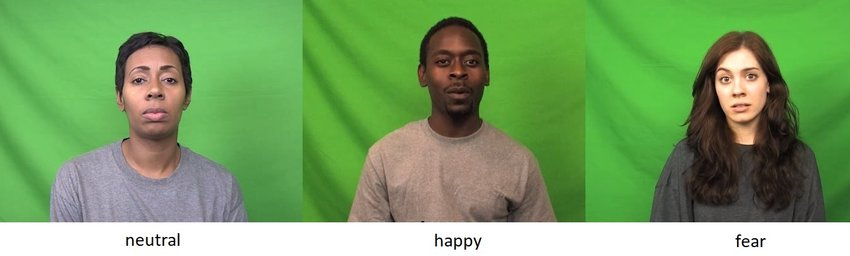
\includegraphics[width=15cm]{./content/images/crema-d_img.jpg}
    \caption{Ảnh được cắt từ các video trong tập dữ liệu \textit{CREMA-D}}
    \label{fig:sample-rapv1}
\end{figure}

\begin{figure}[H]
    \centering
    
\includegraphics[width=15cm]{./content/images/lrw_img.png}
    \caption{Ảnh được cắt từ các video trong tập dữ liệu \textit{LRW}}
    \label{fig:sample-rapv1}
\end{figure}

\begin{figure}[H]
    \centering
    
\includegraphics[width=15cm]{./content/images/vox_img.png}
    \caption{Ảnh được cắt từ các video trong tập dữ liệu \textit{VoxCeleb}}
    \label{fig:sample-rapv1}
\end{figure}

\subsection{\texorpdfstring{Các thí nghiệm dự kiến sẽ triển khai}{Empty}}

Nhằm mục đích khảo sát, kiểm định và học hỏi, kế thừa các ý tưởng từ các nghiên cứu trước, tác giả sẽ đọc hiểu ý tưởng từ các bài báo từ năm 2018 trở lại đây để nắm rõ lý thuyết và cách vận hành của mô hình được đề ra. Sau đó cài đặt, tiến hành lại các thí nghiệm trên để kiểm chứng và học hỏi thêm kinh nghiệm, đồng thời sẽ cố gắng đề ra những cải tiến cho các mô hình trên nhằm mục đích tăng chất lượng hình ảnh và tính đồng bộ âm thanh cho video được tạo sinh. Từ việc thử nghiệm, cải tiến các mô hình của các nghiên cứu trước, tác giả sẽ thiết kế các mô hình mới và tiến hành thử nghiệm với những cài đặt siêu tham số khác nhau.

\section{\texorpdfstring{Kế hoạch triển khai}{Plan}}
\section{\texorpdfstring{Tổng quan các công trình nghiên cứu liên quan}{Content}}
Việc tạo sinh dữ liệu mới trong thời gian gần đây đã phát triển mạnh mẽ với sự ra đời của kiến trúc mạng GANs. Hệ thống mạng GANs bao gồm các mạng học máy, học sâu nhỏ hơn, chia thành hai thành phân là mạng tạo sinh dữ liệu (mạng G) và mạng phân biệt dữ liệu (mạng D). Mạng G đóng vai trò như một Variational Autoencoder \cite{vae_base},  có chức năng học và xấp xỉ được phân phối xác suất của dữ liệu gốc, từ đó tạo sinh ra dữ liệu mới giữ được đặc trưng và tương đồng với dữ liệu gốc. Mạng D có chức năng phân biệt giữa dữ liệu được tạo sinh bởi mạng G và tập dữ liệu huấn luyện. Trong quá trình huấn luyện, dựa trên hàm mất mát của D, các trọng số của cả hai mạng G và D đều được cập nhật trong quá trình lan truyền ngược, từ đó giúp hai mạng này tăng độ chính xác. Với mạng G, qua quá trình huấn luyện, mạng sẽ có khả năng tạo sinh ra được dữ liệu ngày càng chân thực hơn, khó phân biệt hơn. Trong khi đó, mạng D cũng ngày càng có chức năng phân biệt tốt hơn, chuẩn xác hơn. Đến một lúc nào đó, độ chính xác của hai mạng sẽ đạt đến mức cân bằng, lúc này hai mạng đã hội tụ và không thể được cải thiện hơn với kiến trúc mạng và tập dữ liệu huấn luyện hiện tại, nên ta sẽ dừng quá trình huấn luyện tại đây.

\section{\texorpdfstring{Nội dung dự kiến của luận văn}{Conclusion}}

Luận văn tốt nghiệp sẽ được chia thành các phần như sau:

\textit{Lời cam đoan của tác giả}: Cam đoan các công việc, thử nghiệm và kết quả được đưa ra trong luận văn là trung thực, khách quan.

\textit{Tóm tắt luận văn}: Trình bày ngắn gọn về cấu trúc của Luận văn, giới thiệu những điểm nhấn của Luận văn, kết quả, và các từ khóa đi kèm.

\textit{Mở đầu}: Nêu lý do chọn đề tài, mục đích, đối tượng và phạm vi nghiên cứu, ý nghĩa khoa học và ý nghĩa thực tiễn của đề tài.

\textit{Tổng quan tình hình nghiên cứu, mục tiêu và nhiệm vụ nghiên cứu}: Sơ lược, phân tích, đánh giá các công trình nghiên cứu nổi tiếng có liên quan đến đề tài. Nêu những vấn đề bức thiết cần phải giải quyết, chỉ ra những thiếu sót mà những nghiên cứu trước đây chưa giải quyết được.

\textit{Cơ sở lý thuyết}: Trình bày cơ sở lý thuyết, các lập luận, căn cứ khoa học được sử dụng trong Luận văn.

\textit{Phương pháp nghiên cứu}: Trình bày chi tiết về ý tưởng, các mô hình toán, các chứng minh nếu có. Đồng thời trình bày các bước thực hiện và khảo sát, kiểm nghiệm kết quả nghiên cứu. Mô tả kết quả nghiên cứu khi thử nghiệm với nhiều tập dữ liệu và những độ khó khác nhau.

\textit{Kết quả nghiên cứu}: Mô tả ngắn gọn các kết quả nghiên cứu, thực nghiệm. Bàn luận về điểm mạnh, điểm yếu của mô hình được xây dựng trong luận văn. So sánh kết quả thu được trong quá trình nghiên cứu, thực nghiệm của đề tài và đối chiếu với kết quả nghiên cứu, thực nghiệm của các tác giả khác một cách khách quan. Nêu lên điểm nổi bật, khác biệt của luận văn đối với các nghiên cứu khác.

\textit{Kết luận và hướng nghiên cứu mở rộng đề tài}: Mô tả, bình luận ngắn gọn và đưa ra kết luận về kết quả nghiên cứu của luận văn và cách thức áp dụng thực tiễn. Đề ra các hướng nghiên cứu mở rộng cho Luận văn.

\textit{Danh mục tài liệu tham khảo}: Trích dẫn các tài liệu được sử dụng trong Luận văn.

\section{\texorpdfstring{Kết luận}{Plan}}

Qua đề cương Luận văn, tác giả đã tìm hiểu thêm nhiều kiến thức và học hỏi được các ý tưởng, phương pháp mà các nghiên cứu khác đã áp dụng. Qua đó đề ra một số ý tưởng nghiên cứu riêng cho Luận văn. Luận văn tốt nghiệp sẽ được thực hiện nhằm mục đích giải quyết các vấn đề còn tồn tại của việc tạo sinh hình ảnh gương mặt người đang nói, cố gắng cải thiện chất lượng hình ảnh và thêm vào đó các chuyển động khác như chuyển động của đầu, tóc hay các cơ trên mặt theo cảm xúc người nói. Luận văn cũng sẽ đề ra cách để cải thiện vùng hình ảnh ngoài gương mặt để video được tạo ra chân thực nhất có thể. Để làm được điều này, Luận văn sẽ xem xét và phân tích gương mặt trong không gian ba chiều thay vì hai chiều như trước đây, vì không gian ba chiều cho phép giả lập chuyển động của đầu. Đồng thời cũng sẽ thiết kế một kiến trúc mới có chức năng học và tạo sinh các thông số đê sinh ảnh cho một người nhất định.

\bibliographystyle{unsrt}
\bibliography{references}
\appendix
\include{./references}
\end{document}